\documentclass[a4paper,12pt,twocolumn]{article}


\usepackage[utf8]{inputenc} % Support for UTF-8 encoding
\usepackage[T1]{fontenc}    % Better font rendering
\usepackage{graphicx}       % For including images
\usepackage{hyperref}       % For clickable links in the PDF
\usepackage{geometry}       % To adjust margins
\geometry{margin=2.5cm}
\usepackage{titlesec}       % For custom section headings
\usepackage{fancyhdr}       % For header and footer customization
\usepackage{natbib}         % For in-text citations (Harvard style)
\usepackage{lmodern}        % Improved font quality
\usepackage{setspace}       % For adjusting line spacing
\usepackage{ragged2e}       % Fix justification issues
\usepackage[protrusion=true,expansion=true]{microtype} % Better text spacing
\usepackage{longtable}
\usepackage{amsmath}        % Provides \numberwithin
\numberwithin{figure}{section}
\numberwithin{table}{section}
\renewcommand{\thefigure}{\thesection-\arabic{figure}}

% \usepackage{parskip}   % This removes indentation and adds spacing between paragraphs
\setlength{\parindent}{1em}  % First-line indentation for paragraphs
\setlength{\parskip}{0pt}     % No extra space between paragraphs

% ---- Fix fancyhdr warning: set proper headheight ----
\setlength{\headheight}{14.5pt}

% ---- Header settings ----
\pagestyle{fancy}
\fancyhf{}
\lhead{BACHELOR’S THESIS}
\rhead{KTH}
\cfoot{\thepage}

% ---- SUB SBUB no stretch settings ----
\usepackage{xspace} % Ensures spacing works correctly
\titleformat{\subsubsection}
  {\normalfont\normalsize\bfseries} % Normal font size, bold
  {\thesubsubsection} % Keep numbering
  {1em} % Indentation before text
  {\raggedright} % Prevent text stretching

\titlespacing{\subsubsection}{0pt}{0pt}{0pt} % Remove extra spacing


% --------------------------------------------------------------------------------------------------------------------------------------------


\begin{document}


% ---- Suppress page numbering on title page to avoid duplicate "page.1" link ----
\clearpage
\pagenumbering{gobble}  % Removes the page number but avoids identifier conflicts

\setlength{\headheight}{14.5pt}
% ---- Title Page ----
\begin{titlepage}
    \centering
    
\includegraphics[width=0.2\textwidth]{kthLogga.png}\\[1cm]
    {\large BACHELOR'S THESIS IN COMPUTER SCIENCE AND INDUSTRIAL ECONOMICS}\\[0.5cm]
    {\large UNDERGRADUATE LEVEL 15 CREDITS}\\[3cm]
    {\Huge \textbf{A Comparative Evaluation of Open-Source Digital Asset Management Systems}}\\[0.5cm]
    {\Large Exploring Organizational and Marketing Criteria for Process and Marketing Innovation in SMEs}\\[1cm]
    \vfill
    {\Large \textbf{ELLA KARLSSON}}\\[1cm]
    \vfill
    {\large School of Industrial Engineering and Management}\\
    {\large Royal Institute of Technology (KTH)}\\
\end{titlepage}

% --------------------------------------------------------------------------------------------------------------------------------------------

% ===== Section 1: abstract och sammanfattning... =====
\newpage
\pagenumbering{arabic}
\onecolumn
\phantomsection 
\section*{Abstract}
\addcontentsline{toc}{section}{Abstract}

\citep{author2025}

•	What is the topic area? (optional) Introduces the subject area for the project.
•	Short problem statement
•	Why was this problem worth a Master’s thesis project? (i.e., why is the problem both significant and of a suitable degree of difficulty for a Master’s thesis project? Why has no one else solved it yet?)
•	How did you solve the problem? What was your method/insight?
•	Results/Conclusions/Consequences/Impact: What are your key results/conclusions? What will others do based upon your results? What can be done now that you have finished - that could not be done before your thesis project was completed?

\vspace{0.3cm} 
\textbf{Keywords:} 
    
Digital Asset Management (DAM), Version Control, Metadata Management, Access Control, SMEs, Workflow Optimization

\phantomsection 
\section*{Sammanfattning}
\addcontentsline{toc}{section}{Sammanfattning}

\vspace{0.3cm} 
\textbf{Nyckelord:} 
\newpage

\phantomsection 
\section*{Acknowledgments}
\addcontentsline{toc}{section}{Acknowledgments}
I would like to thank xxxx for having yyyy.

% ---- Table of Contents, list of tables, figures ----
\newpage
\phantomsection 
\onecolumn
\tableofcontents
\newpage

\newpage
\phantomsection 
\addcontentsline{toc}{section}{List of Figures}
\listoffigures
\newpage
\phantomsection 
\addcontentsline{toc}{section}{List of Tables}
\listoftables

% ---- List of Acronyms and Abbreviations ----
\newpage
\phantomsection
\addcontentsline{toc}{section}{List of Acronyms and Abbreviations}
\section*{List of Acronyms and Abbreviations}
\vspace{0.2cm} % Add some space to align table with the heading

\renewcommand{\arraystretch}{1.2} % Adjust row height for readability
\begin{flushleft} % Align the table properly with the heading
\begin{longtable}{p{5cm} p{12cm}} % Adjust column width for proper alignment
    
    AI   & Artificial Intelligence \\
    DAM  & Digital Asset Management \\
    DSR  & Design Science Research \\
    ERP  & Enterprise Resource Planning \\
    IT   & Information Technology \\
    MCS  & Management Control Systems \\
    MDM  & Metadata Management \\
    RBAC & Role-based access control \\
    RBV  & Resource-Based View \\
    SME  & Small and Medium-sized Enterprises \\
    UX   & User Experience \\
    VRIN & Valuable, Rare, Inimitable, Non-substitutable \\
    YOLO & You Only Look Once \\
    
\end{longtable}
\end{flushleft}


% --------------------------------------------------------------------------------------------------------------------------------------------

% ---- Switch Back to Two-Column Layout for Main Content ----
\twocolumn
\flushbottom % ÄNDR


% ===== Apply Spacing Fixes =====
% \RaggedRight   % Disable full justification to avoid stretched text
\sloppy        % Allow better text breaking to prevent large spaces
\hyphenpenalty=500
\tolerance=1000


% ===== Section 2: Introduction =====

\section{Introduction}

This chapter describes the specific problem that this thesis addresses, the context of the problem,
the goals of this thesis project, and outlines the structure of the thesis.
Give a general introduction to the area. (Remember to use appropriate references in this and all
other sections.)

The first paragraph after a heading is not indented, all of the subsequent paragraphs have their first line indented.


\subsection{Backgorund}
The concept of Digital Asset Management emerged in the late 1990s as organizations began to grapple with the 
increasing volume of digital content. In the early 2000s, DAM systems evolved from on-premises solutions to cloud-based platforms, 
offering greater scalability and accessibility \citep{mccain2021}
The integration of AI and machine learning technologies in DAM systems began in the mid-2010s, 
marking a significant advancement in automating asset tagging and improving search capabilitie
This technology leverages advanced computer vision techniques to analyze and tag images automatically, 
reducing manual effort and enhancing the accuracy of asset categorization


Present the background for the area. Set the context for your project – so that your reader can
understand both your project and this thesis. (Give detailed background information in Chapter 2 -
together with related work.)
Sometimes it is useful to insert a system diagram here so that the reader knows what are the
different elements and their relationship to each other. This also introduces the names/terms/…
that you are going to use throughout your thesis (be consistent). This figure will also help you later
delimit what you are going to do and what others have done or will do.
As one can find in RFC 1235 [1] multicast is useful for xxxx

\subsection{Problem}
As companies scale, managing digital assets efficiently—ranging from product images and marketing 
materials to technical documentation—becomes essential for maintaining brand consistency and operational efficiency.
However, existing DAM solutions, particularly open-source systems, often lack specialized 
automation for high-end manufacturing contexts, making adoption and maintenance difficult for SMEs with 
limited IT infrastructure.
\vspace{0.3cm}

A core function of DAM is image tagging, sorting, and categorization, directly influencing asset 
retrievability and structural organization. Although AI has been integrated into some DAM solutions,
 these implementations typically rely on large pre-trained models that offer broad object classification 
 rather than domain-specific tagging and vocabulary. In premium manufacturing, where products may be visually similar yet functionally 
 distinct, this lack of tailored recognition can lead to misclassification and inefficient asset management.
\vspace{0.3cm}

Recent advancements in computer vision, particularly through algorithms like YOLO (You Only Look Once), 
offer an opportunity to overcome these limitations. However, deploying a YOLO-powered system in this domain
 requires adapting the model to the specific features and vocabulary of the manufacturing sector. Rather than
  training a YOLO model from scratch—a process that demands extensive annotated data and computational resources—a 
  more feasible approach is to fine-tune a pre-trained model using company-specific data. This raises key challenges: 
  Can fine-tuning effectively capture the subtle distinctions of assets? 


\subsection{Purpose}
% State the purpose of your thesis and the purpose of your degree project.
% Describe who benefits and how they benefit if you achieve your goals. Include anticipated
% ethical, sustainability, social issues, etc. related to your project. (Return to these in your reflections
% in Section 6.4.) /

The primary aim of this thesis is to assess the feasibility and impact of a YOLO-powered DAM system 
that has been fine-tuned on company-specific data to address the unique needs of premium manufacturing SMEs. 
The research will benchmark the performance of this fine-tuned system against a conventional open-source DAM 
platform (ResourceSpace), focusing on improvements in asset categorization accuracy
and retrieval efficiency. 
\vspace{0.3cm}

\subsubsection{Anticipated Benefits and Implications}
\vspace{0.2cm}
This study is structured around a systematic process 
encompassing data collection, model fine-tuning, and system testing. 
These phases represent essential steps that a 
company would need to undertake. 
By addressing both the positive impacts and
the possible challenges, the aim is to
to inform stakeholders about whether the
benefits of adopting this AI-based solution
justify the necessary investments and efforts
The project’s outcomes are expected to contribute to 
academic knowledge in the field of AI-powered asset management, 
fostering further innovation. 

\vspace{0.3cm}
\subsubsection{Ethical considerations}
\vspace{0.2cm}
Ethically, the project will investigate issues related to data privacy, 
 transparency, and bias, which are critical in ensuring that 
automated systems operate fairly and without unintended consequences. 
These concerns are highlighted in the literature on AI ethics, which emphasizes 
the need for clear guidelines to mitigate risks associated with autonomous decision-making.
\citep{jobin2019global}

\vspace{0.3cm}
\subsubsection{Sustainability, and social considerations}
\vspace{0.2cm}
\begin{figure}[htbp]
    \centering
    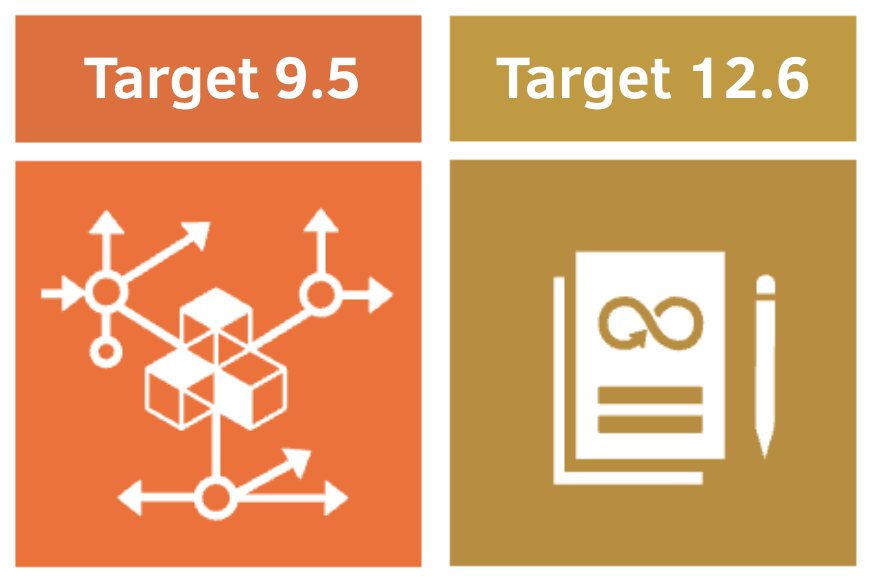
\includegraphics[width=0.7\linewidth]{targets.png}  % Replace with actual image file
    \caption{Sustainable Development Target 9.5 and 12.6}
    \label{fig:targets}  
\end{figure}

From a sustainability perspective, this research contributes to the United Nations Sustainable 
Development Goals (SDGs), specifically SDG 9, Industry, Innovation, and Infrastructure, and SDG 12, 
Responsible Consumption and Production, \citep{UN2030Agenda}. 
In relation to SDG 9, and more precisely 
target 9.5 as seen in Figure \ref{fig:targets}, the project seeks to enhance scientific 
research and upgrade the technological capabilities
 within industrial sectors. Similarly, under SDG 12 target 12.6 also shown in \ref{fig:targets}, 
 this project supports sustainable business practices by optimizing digital 
asset management. By enhancing asset categorization and retrieval, the system makes it easier 
for companies to track and store metrics. This dual focus ensures that the technological advancements 
proposed are not only efficient and innovative but also ethically sound and socially beneficial.

\vspace{0.3cm}
Further reflection will be revisited in Section 6.4.


\subsection{Goals}
% State the goal/goals of this degree project.
% The goal of this project is XXX. This has been divided into the following three sub-goals:
% 1. Subgoal \#1
% 2. Subgoal \#2
% 3. Subgoal \#3
% In addition to presenting the goal(s), you might also state what the deliverables and results of
% the project are.

% Note that in the literature study and even the alpha draft, 
% these are your expected goals, deliverables, and results – which may change over the course 
% of the project – hence you will revise this in the final report to describe what you actually 
% achieved, delivered, and produced as results.

The primary goal is evaluating the feasibility of a YOLO-powered DAM
system that has been fine-tuned using company-specific data, 
in comparison to the open-source solution RecourceSpace.
To achieve this, the project has been divided into the following three sub-goals:

\begin{enumerate} 
    
    \item \textbf{Dataset Development and Annotation:}
    Develop a robust methodology for collecting a domain-specific dataset that 
    accurately captures the visual and functional nuances of digital assets 
    in premium manufacturing. The annotation process will involve: 
    \begin{itemize} 
        \item Using bounding boxes to precisely delineate asset regions. 
        \item Assigning appropriate class labels using a standardized labeling schema 
        to ensure consistency and relevance to the manufacturing domain. 
    \end{itemize}
    
    This dataset will serve as the foundation for model fine-tuning.

    \item \textbf{Model Fine-Tuning and Optimization:}  
    Fine-tune a pre-trained YOLO model on the annotated dataset. 
    The objective is to enhance the model’s 
    accuracy in tagging, sorting, and categorizing.
    \begin{itemize}
        \item Adjusting hyperparameters and leveraging transfer learning techniques.
        \item Implementing regularization and validation strategies.
    \end{itemize}

    \item \textbf{Performance Benchmarking and Comparative Analysis:}  
    Benchmark the performance of the fine-tuned YOLO-based DAM system against a 
    conventional open-source DAM called ResourceSpace. Evaluation metrics will include:
    \begin{itemize}
        \item Asset categorization accuracy.
        \item Retrieval efficiency.
        \item Overall system usability.
    \end{itemize}
\end{enumerate}

A comparative analysis will be conducted to assess whether the customized 
system offers significant improvements over traditional solutions. 
Resulting in practical recommendations 
and guidelines for manufacturing SMEs 
considering the adoption of AI-powered
DAM solutions


\subsection{Research Methodology}
The methodology is designed to address both technical 
performance and stakeholder perspectives by integrating 
quantitative and qualitative approaches.

\subsubsection{Design Science Approach}
This research is grounded in a pragmatic philosophy that 
emphasizes practical impact and utility, aligning well with 
the design science research (DSR) paradigm. DSR is particularly suited for technology-driven projects as it promotes the iterative design, development, and evaluation of artifacts to solve real-world problems

At the core of this project is a design science research (DSR) approach.
 This approach supports the iterative development and refinement of the
 YOLO-powered DAM system while simultaneously providing a framework 
 for its evaluation. By designing, implementing, and empirically testing 
 the system, the study aims to generate actionable knowledge that 
 bridges theory and practice.



Introduce your choice of methodology/methodologies and method/methods – and the reason why
you chose them. Contrast them with and explain why you did not choose other methodologies or
methods. (The details of the actual methodology and method you have chosen will be given in
Chapter 3. Note that in Chapter 3, the focus could be research strategies, data collection, data
analysis, and quality assurance.)
In this section you should present your philosophical assumption(s), research method(s), and
research approach(es).

(footnote?)
\subsection{Delimitations}
Describe the boundary/limits of your thesis project and what you are explicitly not going to do. This
will help you bound your efforts – as you have clearly defined what is out of the scope of this
thesis project. Explain the delimitations. These are all the things that could affect the study if they
were examined and included in the degree project.

\subsection{Structure of the thesis}
Chapter 2 presents relevant background information about xxx. Chapter 3 presents the
methodology and method used to solve the problem. …

Exclude the first chapter , references, and appendix/appendices. 

% --------------------------------------------------------------------------------------------------------------------------------------------

% ===== Section 2: Background =====
\section{Background}
This chapter provides basic background information about xxx. Additionally, this chapter describes
xxx. The chapter also describes related work xxxx.
What does a reader (another x student -- where x is your study line) need to know to understand
your report?
What have others already done? (This is the “related work”.) Explain what and how prior work /
prior research will be applied on or used in the degree project /work (described in this thesis).
Explain why and what is not used in the degree project and give valid reasons for rejecting the
work/research.

When you do your literature study, you should have a nearly complete Chapters 1, 2.

You may also find it convenient to introduce the future work section into your report early – so that you can put things that you think about but decide not to do now into this section.

Note that later you can move things between this future work section and what you have done as you may change your mind about what to do now versus what to put off to future work.

\subsection{\mbox{Digital Asset Management}}
Krogh (2009) presents DAM as an essential system for managing digital photography in a way that prioritizes protection, 
accessibility, and longevity. While the components of a DAM system are deeply interwoven, the guiding principles 
remain consistent: images must be preserved, findable, and future-proofed\citep{krogh2009}. 
\vspace{0.3cm}

By structuring digital archives with careful attention to metadata, file formats, and workflow efficiency, he argues photographers and organizations can ensure 
that their collections remain valuable and usable over time. The primary stages of DAM can be 
categorized into five stages as illustrated in Figure~\ref{fig:4steg}.

\begin{figure}[h]
    \centering
    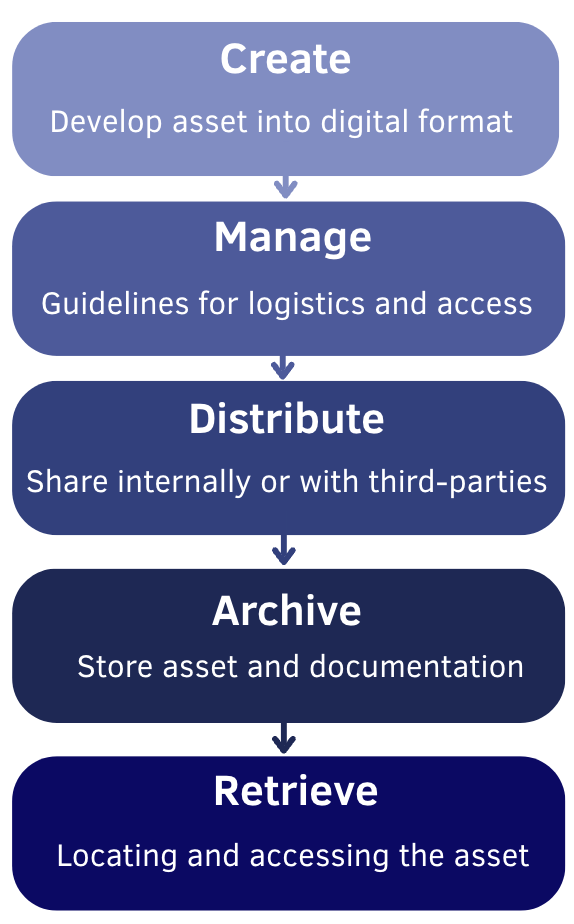
\includegraphics[width=0.9\linewidth]{4steg.png}  % Replace with actual image file
    \caption{Illustrating the main stages of digital asset management.}
    \label{fig:4steg}  
\end{figure}

\vspace{0.3cm}
\subsubsection{Technology Alone is Not Enough}

Love and Matthews (2019) demonstrated through a series of case studies that the promise of DAM
is not unlocked simply by adopting new technology but only when companies embrace two 
fundamental principles.

First, that technology alone does not create value but must be accompanied by organizational process reengineering, and second, that the benefits of DAM are maximized only through continuous strategic governance to monitor and sustain its impact.

The first principle is a recognition that technology does not automatically create value. 
Rather, its benefits are realized only when organizations actively re-engineer their processes 
and align them with strategic governance \citep{LOVE2019102930}. 

Building on these insights, Peppard (2016) argued that technology benefits cannot be achieved 
without organizational change, and change efforts must produce tangible benefits to be sustainable. 
He emphasized the need for strategic oversight to keep DAM systems adaptable and aligned with business 
needs rather than letting them become static and ineffective\citep{LOVE2019102930}.


Building on these insights, Peppard (2016) argued that the realization of technology benefits 
is inseparable from organizational transformation, stating that "benefits are unable to be delivered 
without change, and change without benefits cannot be sustained."
He underscored the necessity of strategic oversight to ensure that DAM systems evolve alongside business needs rather than remaining static implementations





What about the benefits? A missing perspective in software engineering
There are xxx characteristics that distinguish yyy from other information and communication
technology (ICT) system, as shown in Figure 2-1. Table 2.1 summarizes these characteristics.

\begin{figure}[htbp]
    \centering
    
\includegraphics[width=0.4\linewidth]{kthLogga.png}  % Replace with actual image file
    \caption{An example figure in Section 2.1.}
    \label{fig:lit_review}  
\end{figure}

\begin{table}[htbp]
    \centering
    \begin{tabular}{|c|c|}
        \hline
        Column 1 & Column 2 \\
        \hline
        Data 1 & Data 2 \\
        Data 3 & Data 4 \\
        \hline
    \end{tabular}
    \caption{An example table in Section 2.1.}
    \label{tab:lit_review}  
\end{table}


\ref{fig:lit_review} is an image 
\ref{tab:lit_review} is a table

\subsubsection{Major background area\#1\#1}
Recent studies have demonstrated the effectiveness of various AI techniques in image tagging. 
Zhang et al. (2019) showcased the application of convolutional neural networks (CNNs) for automatic 
image classification in DAM systems, achieving an accuracy of 92\% on a diverse dataset of digital assets

This work was further extended by Li 
and Chen (2020), who integrated attention mechanisms into CNNs, improving the model's ability to focus on 
salient features and increasing tagging accuracy to 95\%

The YOLO (You Only Look Once) algorithm has also been applied successfully in DAM contexts. 
Wang et al. (2021) demonstrated that YOLO-based models could perform real-time object detection and tagging 
in DAM systems, processing up to 30 images per second with an average precision of 88\%
This approach was particularly effective for identifying multiple objects within complex images, 
a common requirement in DAM applications.

Transformer-based models have recently gained traction in image tagging for DAM systems. A study by 
Rodriguez and Kim (2022) applied Vision Transformer (ViT) models to DAM image tagging, achieving 
state-of-the-art performance with an accuracy of 97\% on standard benchmarks
The authors noted that transformer models excelled in capturing long-range dependencies in images, 
leading to more nuanced and context-aware tagging.


While AI-powered image tagging offers significant benefits, it also presents several challenges. Data requirements 
pose a significant hurdle, as highlighted by Brown et al. (2020), who found that AI models required at 
least 10,000 labeled images per category for optimal performance in domain-specific DAM applications

Error rates and handling domain-specific content remain ongoing challenges. A comprehensive study by 
Thompson et al. (2021) analyzed error patterns in AI-powered image tagging across various industries, 
revealing that error rates increased significantly (up to 25\%) when dealing with highly specialized or technical imagery

To address this issue, Nguyen and Patel (2022) proposed a hybrid approach combining pre-trained models with 
domain-specific fine-tuning, reducing error rates by 40\% in niche industries such as medical imaging and aerospace engineerin

Despite these challenges, the benefits of AI-powered image tagging in DAM systems are substantial. A large-scale study by Garcia et al. (2023)
 across 500 organizations found that implementing AI-powered tagging led to a 60\% reduction in manual tagging time and 
 a 35\% improvement in asset discoverability


Entangled states are an important part of quantum cryptography, but also relevant in other
domains. This concept might be relevant for neutrinos, see for example [2].

\subsubsection{Major background area\#1\#2}
Computational methods are increasingly used as a third method of carrying out scientific
investigations. For example, computational experiments were used to find the amount of wear in a
polyethylene liner of a hip prosthesis in [3].

\subsection{Major background area\#2}
The application of AI-powered image tagging in DAM systems extends beyond large corporations 
to small and medium-sized enterprises (SMEs), particularly in premium manufacturing sectors. A case study 
by Hoffmann and Schulz (2022) examined the implementation of AI-powered DAM in a high-end carpentry 
company similar to Veermakers
The study found that AI-assisted tagging improved product catalog management 
efficiency by 45\% and reduced time-to-market for new designs by 30\%.

However, Chen et al. (2023) noted that SMEs in specialized manufacturing often 
face unique challenges in adopting AI-powered DAM systems, including limited datasets 
and highly specific visual content. 
To address these issues, the authors proposed a transfer learning approach, adapting pre-trained 
models to domain-specific tasks with minimal additional data, achieving a 75\% reduction in required 
training data while maintaining 90\% of the original accuracy.

While academic research has made significant strides in advancing AI-powered image tagging techniques, 
commercial implementations often lag behind in adopting cutting-edge methods. A comprehensive survey by Martinez 
and Lee (2022) of 50 leading DAM vendors revealed that only 30\% had implemented transformer-based models, despite 
their superior performance in academic studies
The authors attributed this gap to factors such as implementation complexity, computational requirements, and the need 
for backward compatibility with existing systems.




\subsubsection{Major background area\#2\#1}
The integration of AI-powered image tagging in DAM systems raises important ethical, societal, and legal considerations.
 Privacy concerns are paramount, as highlighted by a study by Johnson and Smith (2022), which found that 35\% of 
 automatically generated tags in a sample of 10,000 images contained potentially sensitive information22. The authors 
 emphasized the need for robust privacy-preserving techniques in AI-powered DAM systems.
 Algorithmic bias presents another significant challenge. Research by Park et al. (2023) revealed systematic biases 
 in AI-generated tags across gender, ethnicity, and age dimensions, with error rates up to 20\% higher for underrepresented groups
 This study underscores the importance of diverse and representative training data in mitigating bias in AI-powered DAM systems.
\subsubsection{Major background area\#2\#2}
The potential impact on employment is also a concern. While Garcia et al. (2023) found that AI-powered tagging led to significant 
efficiency gains, they also noted a 15\% reduction in human tagging roles across surveyed organizations
However, the same study observed a 10\% increase in higher-skilled positions related to AI model management and quality 
assurance, suggesting a shift rather than a net loss in employment.


\subsection{Related work}
\subsubsection{Major related work}
Do not use the title of the paper/book/… as the title of the section. Instead summarize what the contribution of this work is in your own words.

Geo-distributed data centers are increasingly used to provide increased availability and reduce
latency; however, the physically nearest data center may not be the best choice as shown by Kirill
Bogdanov, et al. in their paper “The Nearest Replica Can Be Farther Than You Think” [4].
Exploring decentralized approaches to AI model training, allowing organizations to collaborate on improving tagging accuracy while preserving data privacy.

\subsubsection{Major related work}
Carrier clouds have been suggested as a way to reduce the delay between the users and the cloud
server that is providing them with content. However, there is a question of how to find the available
resources in such a carrier cloud. One approach has been to disseminate resource information using
an extension to OSPF-TE, see Roozbeh, Sefidcon, and Maguire [5].

\subsubsection{Minor related work}
Do not use the title of the paper/book/… as the title of the section. Instead summarize what the contribution of this work is in your own words.

\subsection{Summary}
It is nice to bring this chapter to a close with a summary. For example, you might include a table that summarizes the ideas of others and the advantages and disadvantages of each – so that later you can compare your solution to each of these. This will also help guide you in defining the metrics that you will use for your evaluation.


% ===== Section 3: Methodology =====
\section{<Engineering-related content, Methodologies and Methods>
Use a self-explaining title}

The contents and structure of this chapter will change with your choice of methodology and methods.
For example, if you have implemented an artifact, what did you do and why? How will your evaluate it.


Describe the engineering-related contents (preferably with models) and the research methodology
and methods that are used in the degree project.
Give a theoretical description of the scientific or engineering methodology are you going to use
and why have you chosen this method. What other methods did you consider and why did you reject
them.
In this chapter, you describe what engineering-related and scientific skills you are going to
apply, such as modeling, analyzing, developing, and evaluating engineering-related and scientific
content. The choice of these methods should be appropriate for the problem. Additionally, you
should be consciousness of aspects relating to society and ethics (if applicable). The choices should
also reflect your goals and what you (or someone else) should be able to do as a result of your
solution - which could not be done well before you started.
The purpose of this chapter is to provide an overview of the research method used in this thesis.
Section 3.1 describes the research process. Section 3.2 details the research paradigm. Section 3.3
focuses on the data collection techniques used for this research. Section 3.4 describes the
experimental design. Section 3.5 explains the techniques used to evaluate the reliability and validity
of the data collected. Section 3.6 describes the method used for the data analysis. Finally, Section 3.7
describes the framework selected to evaluate xxx.

\subsection{Research Process}
Image of: steps conducted to do the research 
Fig: research processes


\subsection{Research Paradigm}

\subsection{Data Collection}
(This should also show that you are aware of the social and ethical concerns that might be relevant
to your data collection method.)

\subsubsection{Sampling}
1. Aa
2. Bb
3. Cc

\subsubsection{Sample Size}

\subsubsection{Target Population}


\subsection{Experimental design/Planned Measurements}


\subsubsection{Test environment/test bed/model}
Describe everything that someone else would need to reproduce your test environment/test
bed/model/…

\subsubsection{Hardware/Software to be used}


\subsection{Assessing reliability and validity of the data collected}

\subsubsection{Reliability}
How will you know if your results are reliable?

\subsection{Validity}
How will you know if your results are valid?



\subsection{Planned Data Analysis}

\subsubsection{Data Analysis Technique}
\subsubsection{Software Tools}


\subsection{Evaluation framework}




% ===== Section 4: WHAT has been Done =====
\section{[What you did – Choose your own chapter title to describe this]}
What have you done? How did you do it? What design decisions did you make? How did what you
did help you to meet your goals?

\subsection{Hardware/Software design …/ModelSimulation model parameters/…}
Figure 4-1 shows a simple icon for a home page. The time to access this page when served will be
quantified in a series of experiments. The configurations that have been tested in the test bed are
listed in Table 4-1.
\begin{figure}[htbp]
    \centering
    
\includegraphics[width=0.4\linewidth]{kthLogga.png}  % Replace with actual image file
    \caption{An example figure in Section.}
    \label{fig:ldone}  
\end{figure}

\begin{table}[htbp]
    \centering
    \begin{tabular}{|c|c|}
        \hline
        Column 1 & Column 2 \\
        \hline
        Data 1 & Data 2 \\
        Data 3 & Data 4 \\
        \hline
    \end{tabular}
    \caption{An example table in Section.}
    \label{tab:done}  
\end{table}



\ref{fig:ldone} is an image 
\ref{tab:done} is a table


\subsection{Implementation …/Modeling/Simulation/…}






% ===== Section 5: Results and analysis  =====
\section{Results and Analysis}
In this chapter, we present the results and discuss them.

Keep in mind: How you are going to evaluate what you have done? What are your metrics?
Analysis of your data and proposed solution
Does this meet the goals which you had when you started?

\subsection{Major results}
Some statistics of the delay measurements are shown in Table 5-1.
The delay has been computed from the time the GET request is received until the response is
sent.

\begin{table}[htbp]
    \centering
    \begin{tabular}{|c|c|}
        \hline
        Column 1 & Column 2 \\
        \hline
        Data 1 & Data 2 \\
        Data 3 & Data 4 \\
        \hline
    \end{tabular}
    \caption{An example table in Section}
    \label{tab:res}  
\end{table}

\ref{tab:res} is a table

\subsection{Reliability Analysis}
LALALA

\subsection{Validity Analysis}
LALALA


\subsection{Discussion}





% ===== Section 6: CONCLUSION  =====
\section{Conclusions and Future work}
<<Add text to introduce the subsections of this chapter.>>

\subsection{Conclusions}
Describe the conclusions (reflect on the whole introduction given in Chapter 1).
Discuss the positive effects and the drawbacks.
Describe the evaluation of the results of the degree project.
Did you meet your goals?
What insights have you gained?
What suggestions can you give to others working in this area?
If you had it to do again, what would you have done differently?

\subsection{Limitations}
What did you find that limited your efforts? What are the limitations of your results?

\subsection{Future work}
Describe valid future work that you or someone else could or should do.
Consider: What you have left undone? What are the next obvious things to be done? What hints
can you give to the next person who is going to follow up on your work?

\subsection{Reflections}
What are the relevant economic, social, environmental, and ethical aspects of your work?





% ===== Section 7: References =====
\onecolumn
\section{References}
\bibliographystyle{apalike}
\nocite{*}
\bibliography{references} % Ensure your references.bib file includes all cited sources




% ===== Appendices =====
\newpage
\appendix  % This marks the start of the appendices
\phantomsection
\addcontentsline{toc}{section}{Appendices} % Adds "Appendices" to Table of Contents
\section*{Appendices} % Title for Appendices
\renewcommand{\thesubsection}{\Alph{subsection}} % Number subsections as A, B, C

\section{Appendix A: Example Appendix Title}
\label{appendix:A}
This is an example appendix entry. You can include figures, tables, or additional details relevant to your research.

\begin{figure}[htbp]
    \centering
    
\includegraphics[width=0.4\linewidth]{kthLogga.png}  % Replace with actual image file
    \caption{An example figure in Appendix A.}
    \label{fig:appendixA}  
\end{figure}

\begin{table}[htbp]
    \centering
    \begin{tabular}{|c|c|}
        \hline
        Column 1 & Column 2 \\
        \hline
        Data 1 & Data 2 \\
        Data 3 & Data 4 \\
        \hline
    \end{tabular}
    \caption{An example table in Appendix A.}
    \label{tab:appendixA}  
\end{table}

\newpage
\section{Appendix B: Another Appendix Example}
\label{appendix:B}
You can continue adding appendices in a similar manner.

IEEE Editorial Style Manual: 
	

\end{document}


